% http://kleinmann.eit.h-da.de/99_ThesisInfos/

\section{Einführung / Problembeschreibung} 
Jemand "`musste"' Josef K. verleumdet haben, denn ohne dass er etwas Böses \cite{Pleisteiner.2007} getan hätte, wurde er eines Morgens verhaftet. »Wie ein Hund!« sagte er, es war, als sollte die Scham ihn überleben \ac{KDE} \cite[S.55ff]{Accardi.2010}. Als Gregor Sams eines Morgens aus unruhigen Träumen erwachte, fand er sich in seinem Bett zu einem ungeheuren Ungeziefer \index{Ungeziefer} verwandelt \cite{Lewis.2010}.
\subsection{Was ist die Motivation?}
\blindtext

\begin{figure}[h]
	\centering 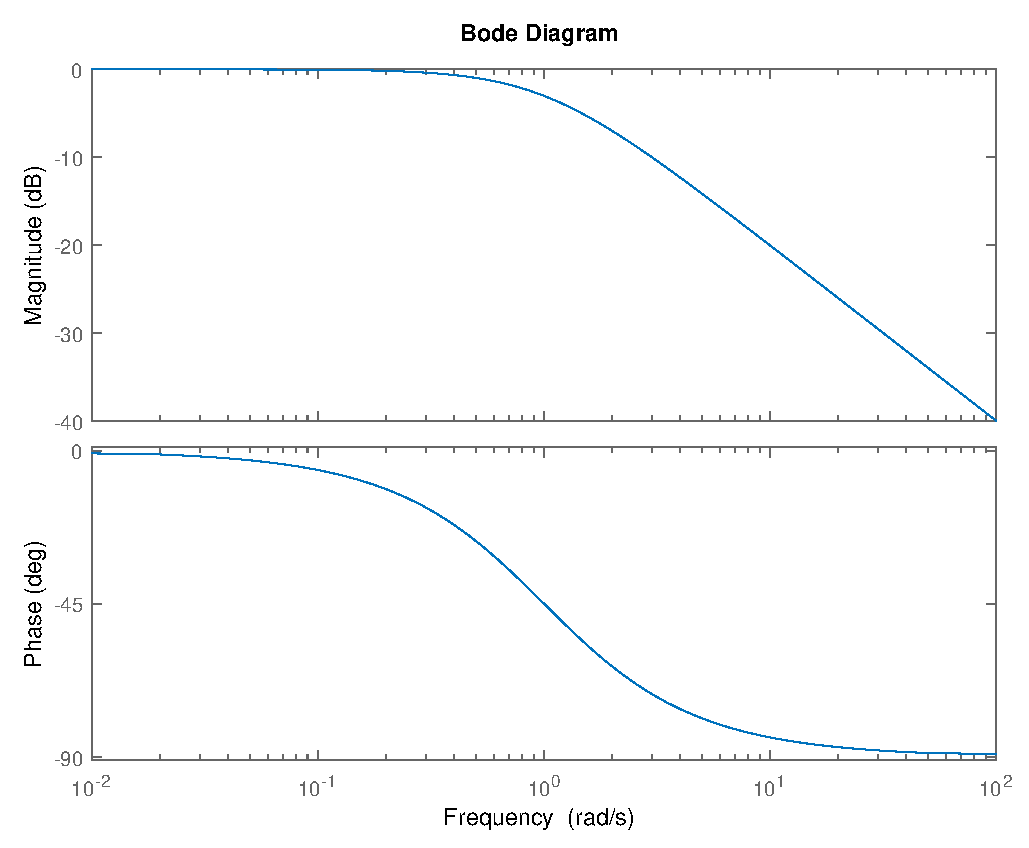
\includegraphics[width=0.5\textwidth]{fig/PT1/PT1.eps}
	\caption{Bodediagramm PT1}
\end{figure}

\blindtext

\begin{IEEEeqnarray}{rCl}
	a & = & b + c \\
	& = & d + e + f + g + h \\
	& = & p + q + r + s
\end{IEEEeqnarray}

\blindtext

\begin{table}[h]
	\centering
	\begin{tabular}[h]{|c|c|}
		\hline
		$U_e$ / V& $U_a$ / V\\ \hline
		0.1 & 0.2 \\ \hline
		0.2 & 0.4 \\ \hline
		0.3 & 0.6 \\ \hline
		0.4 & 0.8 \\ \hline
		0.5 & 1 \\ \hline
	\end{tabular}
	\caption{Messergebnisse}
\end{table}

\subsection{Was ist die Aufgabe?}
\blindtext
\subsection{Was ist das Ziel dieser Arbeit?}
\blindtext
\subsection{Was war der Status Quo, bevor mit dieser Arbeit begonnen wurde?}
\blindtext
\subsubsection{Firma X hat etwas in der Vergangenheit auf diesem oder jenem Wege gemacht…}
\blindtext
\section{Problemlösung}
\blindtext
\subsection{Was sind die Optionen / Welche prinzipiellen Lösungen sind möglich?}
\blindtext
\subsection{Stand der Technik / Wie wird es woanders gemacht?}
\blindtext
\subsection{Was ist der in dieser Arbeit gewählte Ansatz?}
\blindtext
\subsection{Weshalb wurde dieser Ansatz gewählt / Was unterscheidet ihn von anderen / Was ist neu / Was ist bekannt?}
\blindtext
\subsection{Detaillierte Beschreibung der Problemlösung}
\blindtext
\section{Implementierung und Test}
\blindtext
\subsection{Wie wurde es implementiert}
\blindtext
\subsection{Wie wurde getestet}
\blindtext
\subsection{Warum wurde so getestet?}
\blindtext
\section{Validierung}
\blindtext
\subsection{Was sind die Ergebnisse}
\blindtext
\subsection{Vor- und Nachteile des entwickelten Systems}
\blindtext
\section{Zusammenfassung / Fazit / zukünftige Arbeit}
\blindtext
\subsection{Was wurde getan}
\blindtext
\subsection{Was muss noch getan werden / Wie kann das System verbessert werden?}
\blindtext